\documentclass[a4paper]{article}

\usepackage[a4paper,margin=25mm]{geometry}
\usepackage[english]{babel}

\usepackage{parskip} 
\usepackage{microtype}
\usepackage{setspace}
\setstretch{1.2}

\usepackage{tabularx}
\usepackage{booktabs}
\usepackage{multirow}

\usepackage{sectsty}
\sectionfont{\color{AUblueDark}}
\subsectionfont{\color{AUblueDark}}

\usepackage{mathtools, amssymb}
\usepackage{bm}
\renewcommand{\Vec}[1]{\boldsymbol{#1}}
\let\oldhat\hat
\renewcommand{\hat}[1]{\oldhat{\mathbf{#1}}}

\DeclareMathOperator{\grad}{grad}

\usepackage{fourier}

\usepackage[dvipsnames]{xcolor}
\definecolor{AUblue}{RGB}{0,61,115}
\definecolor{AUblueDark}{RGB}{0,37,70}
\definecolor{AUred}{RGB}{226,0,26}
\definecolor{AUyellow}{RGB}{250,187,0}

\usepackage{graphicx}
\graphicspath{{./figures/}}
\usepackage{tikz}
\usetikzlibrary{calc, arrows.meta}

\usepackage{enumitem}
\setlist{topsep=4pt,itemsep=2pt,parsep=0pt}

\usepackage{siunitx}
\sisetup{
  exponent-product = \cdot,
  output-decimal-marker = {,},
  per-mode = fraction,
  round-mode = figures,
  round-precision = 30,
  round-pad = false,
}

%Giles Castelles incfig
\usepackage{import}
\usepackage{xifthen}
\usepackage{pdfpages}
\usepackage{transparent}

\newcommand{\incfig}[2][1]{%
  \def\svgwidth{#1\columnwidth}
  \import{./figures/}{#2.pdf_tex}
}

\usepackage{wrapfig}

\usepackage{fancyhdr}
\pagestyle{fancy}
\fancyhf{}
\renewcommand{\headrule}{\hbox to\headwidth{\color{AUblueDark}\leaders\hrule height 0.6pt\hfill}}
\setlength{\headheight}{20pt}
\fancyhead[L]{\small\AuthorName}
\fancyhead[C]{\small\ReportTitle}
\fancyhead[R]{\small\TheDate}
\usepackage{lastpage}
\fancyfoot[R]{\small p. \thepage{} of \pageref*{LastPage}}
\fancyfoot[L]{\small\CourseName}

\newcommand{\NoteType}{Capstone Project Report}
\newcommand{\Dept}{Department of Mechanical and Production Engineering}
\newcommand{\Uni}{Aarhus University}
\newcommand{\ReportTitle}{\NoteType}
\newcommand{\AuthorName}{Noah Rahbek Bigum Hansen}
\newcommand{\StudentID}{202405538}
\newcommand{\CourseName}{Electromagnetism \& Electronics}
\newcommand{\CourseNumber}{290231U007}
\newcommand{\Course}{\CourseName{} --- \CourseNumber}
\newcommand{\TheDate}{March 16, 2026}
\newcommand{\Logo}{figures/AU}


\usepackage{hyperref}
\hypersetup{
  colorlinks=true,
  linkcolor=AUblue,
  citecolor=AUblue,
  urlcolor=AUblue,
  pdftitle={\NoteType},
  pdfauthor={\AuthorName},
  pdfsubject={\NoteType by \AuthorName{} (\StudentID) for the course \CourseName{} taught at the \Dept{} of \Uni. Last updated on \TheDate{}.},
  pdfcreator={pdfTeX + newtx},
}

\newcommand{\mref}[1]{\hyperref[#1]{\ref*{#1}~\nameref*{#1}}}
\newcommand{\Mref}[1]{\hyperref[#1]{\ref*{#1}~\nameref*{#1}}}

\usepackage[nameinlink,noabbrev]{cleveref}
\usepackage{chngcntr}

\crefname{pluralequation}{equations}{equations}
\Crefname{pluralequation}{Equations}{Equations}

\usepackage{caption}
\captionsetup{font=small}
\usepackage{subcaption} 

\newcommand{\AUheading}[1]{%
  \par\vspace{.4\baselineskip}%
  {\sffamily\bfseries\color{AUred}#1\par}%
  \nobreak%
}

\begin{document}
  \begin{titlepage}
\thispagestyle{empty}
\onehalfspacing

\begin{tikzpicture}[remember picture,overlay]
  \fill[AUblue] ([xshift=-8mm]current page.west |- current page.north)
       rectangle ([xshift=7mm]current page.west |- current page.south);
\end{tikzpicture}

{\large\bfseries \Dept}\\[2pt]
{\normalsize \Uni}
\hfill

\vspace{28mm}
{\fontsize{30pt}{32pt}\selectfont\bfseries \ReportTitle\par}
\vspace{12mm}
{\color{AUblueDark}\rule{\linewidth}{1.5pt}}

\begin{tabular}{@{}ll}
  \textbf{Author:}     & {\AuthorName} \\
  \textbf{Student ID:} & {\StudentID} \\
\textbf{Course:}     & \Course \\
\textbf{Date:}       & \TheDate \\
\end{tabular}

\begin{tikzpicture}[remember picture,overlay]
  \node[anchor=center, inner sep=0] at
    ($ (current page.center) + (0mm, -35mm) $)
    {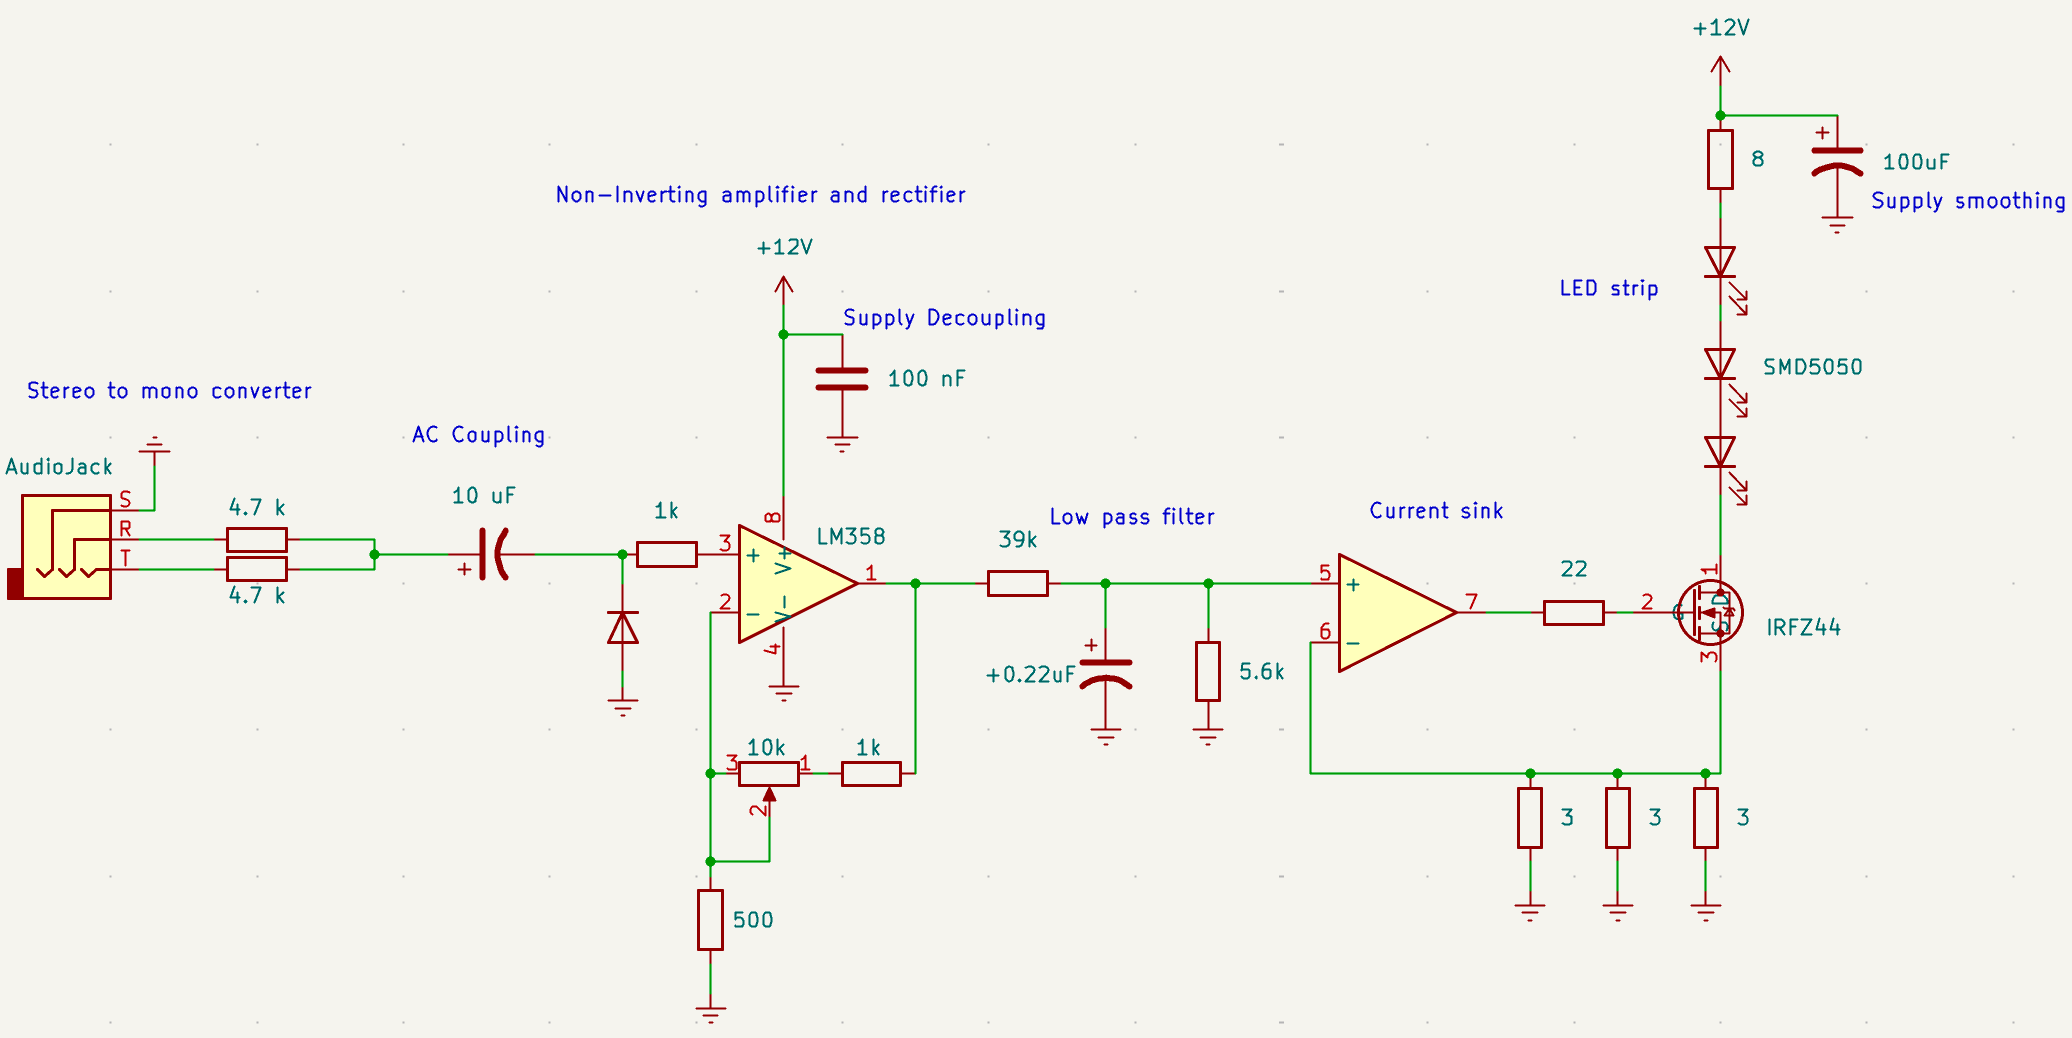
\includegraphics[width=\linewidth]{LEDsysOverview.png}};
\end{tikzpicture}


\begin{tikzpicture}[remember picture,overlay]
  \node[anchor=south east, inner sep=0] at
    ($ (current page.south east) + (-20mm, 20mm) $)
    {\includegraphics[width=42mm]{\Logo}};
\end{tikzpicture}

\vfill
\end{titlepage}

  \newpage

  \section{General Idea}
  For the Capstone project, it was decided that it would be interesting to build an audio-reactive LED circuit.
  The purpose of the circuit is to take an audio signal as input and use it to control the brightness of an LED strip in a way that follows the intensity of the sound.
  The idea for the circuit was inspired by the lights in some modern speakers that ``flicker'' rhythmically with the music.
  The circuit first combines a stereo audio input into a single mono signal, which is  then AC
coupled, amplified, and low-pass filtered.
  This voltage is then used in a current sink stage to regulate the current through an LED strip, thereby adjusting its brightness. 
  The aim is to achieve a responsive and visually clear audio-controlled lighting effect without the need for any programming or any sort of digital controlling.

  \section{Materials}

  \begin{table}[htpb]
  \centering
  \caption{Bill of Materials}
  \label{tab:BOM}
  \begin{tabular}{|c|c|c|}
  \hline
  \textbf{Component Type}     & \textbf{Value} & \textbf{Amount} \\ \hline
  \multirow{6}{*}{Resistors}  & \qty{3}{\ohm}   & 3 \\ \cline{2-3} 
                              & \qty{22}{\ohm}  & 1 \\ \cline{2-3} 
                              & \qty{500}{\ohm} & 1 \\ \cline{2-3} 
                              & \qty{1}{\kilo\ohm}   & 2 \\ \cline{2-3} 
                              & \qty{4,7}{\kilo\ohm} & 2 \\ \cline{2-3} 
                              & \qty{39}{\kilo\ohm}  & 1 \\ \hline
  \multirow{4}{*}{Capacitors} & \qty{100}{\nano\farad}  & 1 \\ \cline{2-3} 
                              & \qty{220}{\nano\farad}  & 1 \\ \cline{2-3} 
                              & \qty{10}{\micro\farad}  & 1 \\ \cline{2-3} 
                              & \qty{100}{\micro\farad} & 1 \\ \hline
  MOSFET                      & IRFZ44  & 1 \\ \hline
  Diode                       & 1N4005  & 1 \\ \hline
  Opamp                       & LM358   & 1 \\ \hline
  LED-Strip                   & SMD5050 & 1 \\ \hline
  RCA-input jack              & ---     & 1 \\ \hline
  \end{tabular}
  \end{table}

  \section{Circuit}
  In the following section the circuit will be explained through the 4 different ``subcircuits'' that the circuit is composed of. These are the input stage, the amplification stage, the low pass filtering, and the Current sink and LED control.

  \subsection{Input Stage}
  On \Cref{fig:LEDsysInput} the input stage of the circuit is shown.
  As the circuit is mounted to a TV, the audio jack on the figure is not representative of how the audio input is actually delivered.
  Instead of the audio jack the audio output of the TV is gathered through the SCARD output, where a DAC converts the signal to an analog audio signal which is then transmitted to the circuit using two RCA cables.

  \begin{wrapfigure}{r}{0.4\linewidth}
    \centering
    \vspace{-1.2\baselineskip}
    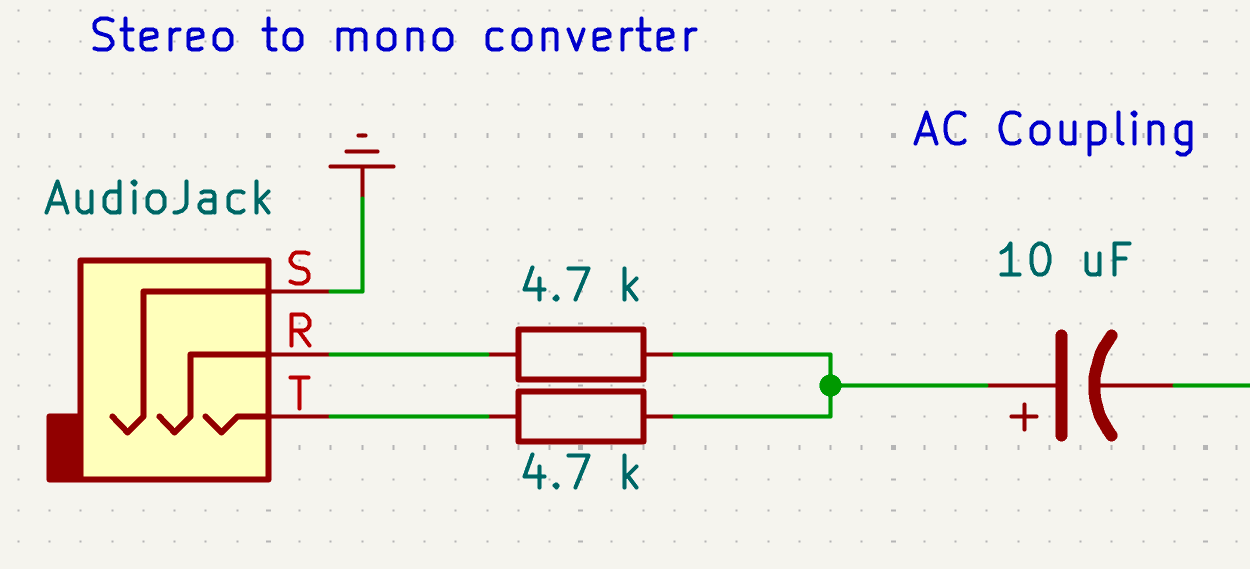
\includegraphics[width=\linewidth]{./figures/LEDsysInput.png}
    \caption{Input stage of the Circuit.}
    \label{fig:LEDsysInput}
\end{wrapfigure}

  These two audio cables are represented as the ring and tip (R and T) connections of the audio jack on \Cref{fig:LEDsysInput}.
  As we are not interested in any stereo activity there might be happening in the audio, the two stereo signals are converted into a single mono signal through two \qty{4,7}{\kilo\ohm} resistors.
  The resistors are added here to avoid shorting the two signals, which could produce large currents between the signal paths and poor signal quality if the voltage of the two stereo signals ever were to become too large.
  After the stereo to mono conversion the signal is passed through a \qty{10}{\micro\farad} capacitor to remove any DC-offset that might have been present in the signal.
  This is done to make the following opamp-stage only responds to the AC-waveform and not any DC-effects.

  \subsection{Amplification}
  As shown on \Cref{fig:LEDsysAmp}, the signal is then partially clamped to ground through a diode (in this case a 1N4005).
  This is done to protect the LM358-opamp from input voltages too far lower than \qty{0}{\V}, as the opamp is only powered from \qty{0}{\V} to \qty{12}{\V} by the supply.

    
  \begin{wrapfigure}{r}{0.4\linewidth}
    \centering
    \vspace{-1.2\baselineskip}
    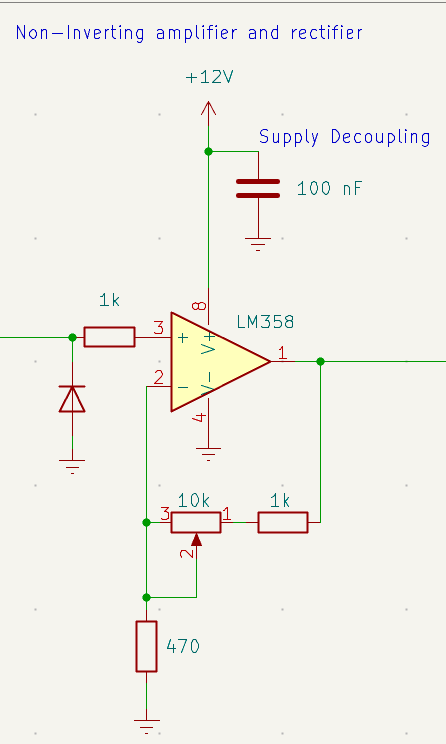
\includegraphics[width=\linewidth]{./figures/LEDsysAmp.png}
    \caption{Amplification stage of the circuit.}
    \label{fig:LEDsysAmp}
  \end{wrapfigure}

  Then the signal is amplified through an LM358-opamp configured as a non-inverting amplifier.
  This IC is powered from a 12V source and is decoupled by a \qty{100}{\nano\farad} capacitor to smooth out any disturbances in the power-supply.
  For a non-inverting amplifier the gain formula is
  \begin{equation*}
    A_v = 1 + \frac{R_f}{R_g}
  \end{equation*}
  where $R_f$ is the feedback resistance and $R_g$ is the resistance from the inverting input to ground.

  Here, a potentiometer was added allowing for adjusting the gain.
  This was done as tests showed that different audio sources delivered their line-level outputs at wildly different voltages leading to a need to be able to compensate for this lower voltage through a higher gain.
  When the pot is at \qty{0}{\ohm} the gain is
  \begin{equation*}
    A_v = 1 + \frac{\qty{1000}{\ohm} }{\qty{470}{\ohm}} = \num{3,12} 
  \end{equation*}
  and when the pot is at \qty{10}{\kilo\ohm} the gain is
  \begin{equation*}
    A_v = 1 + \frac{\qty{11}{\kilo\ohm} }{\qty{470}{\ohm}} = \num{24,4} 
  .\end{equation*}
  Therefore the potentiometer allows the gain to vary from \num{3,1} -- \num{24,4}, which gives ample opportunity for adjusting the gain for different sources. 

  \subsection{Low-pass filtering}
  After the signal has been amplified the low-pass filter shown on \Cref{fig:LEDsysLPF} is used to roll off the higher audio frequencies to avoid excessive light-flickering and instead get a smoother lower frequency response.

  \begin{wrapfigure}{r}{0.3\linewidth}
    \centering
    \vspace{-1.2\baselineskip}
    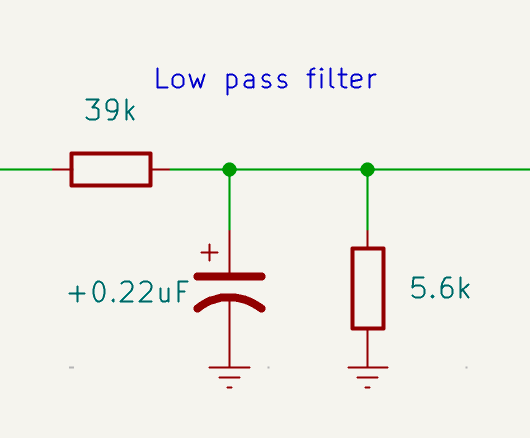
\includegraphics[width=\linewidth]{./figures/LEDsysLPF.png}
    \caption{Low Pass filter stage of the circuit.}
    \label{fig:LEDsysLPF}
  \end{wrapfigure}

  This is not just an ordinary Low-pass filter, however as the \qty{5,6}{\kilo\ohm} resistor is also tied to ground after the ``ordinary'' low-pass filter.
  This resistance to ground allows some of the signal to be filtered to ground leading to overall attenuation of the signal.
  This is done as the amplified signal from the opamp is typically too large, but smaller pots allowing for smaller gain adjustments were not available.

  To find the actual cutoff frequency of this we must consider the overall resistance seen by the capacitor.
  In this case this is $R_{\mathrm{eff}} = \qty{39}{\kilo\ohm} || \qty{5,6}{\kilo\ohm} = \qty{4897}{\ohm}$.

  Then the cutoff frequency can be calculated as
  \begin{equation*}
    f_c = \frac{1}{2 \pi R_{\mathrm{eff}} C} = \frac{1}{2 \pi \cdot \qty{4897}{\ohm} \cdot \qty{220}{\nano\farad} } = \qty{148}{\Hz} 
  .\end{equation*}
  
  The overall signal attenuation caused by the \qty{5,6}{\kilo\ohm} resistor can be found from the voltage-divider formula as
  \begin{align*}
    V_{\mathrm{out}} &= V_{\mathrm{in}} \frac{R}{R_{\mathrm{tot}}} \\
    \frac{V_{\mathrm{out}}}{V_{\mathrm{in}}} &= \frac{R}{R_{\mathrm{tot}}} \\
    &= \frac{\qty{5,6}{\kilo\ohm} }{\qty{44,6}{\kilo\ohm}} \\
    &= \num{0,126}
  .\end{align*}
  Hence, the output signal after the Low-pass filter will \num{0,126} times as large as the input signal for low frequencies and subsequently smaller for larger input frequencies.

  \subsection{Current Sink and LED control}
  The filtered signal is then passed to the other channel of the LM358 opamp.
  Here, the control voltage delivered to the non-inverting input is the filtered signal and the inverting input is the voltage across the three \qty{3}{\ohm} sense resistors shown on \Cref{fig:LEDsysOut} ($R_{\mathrm{S}} = \qty{3}{\ohm} || \qty{3}{\ohm} || \qty{3}{\ohm}  = \qty{1}{\ohm} $).

  
  \begin{wrapfigure}{r}{0.5\linewidth}
    \centering
    \vspace{-1.2\baselineskip}
    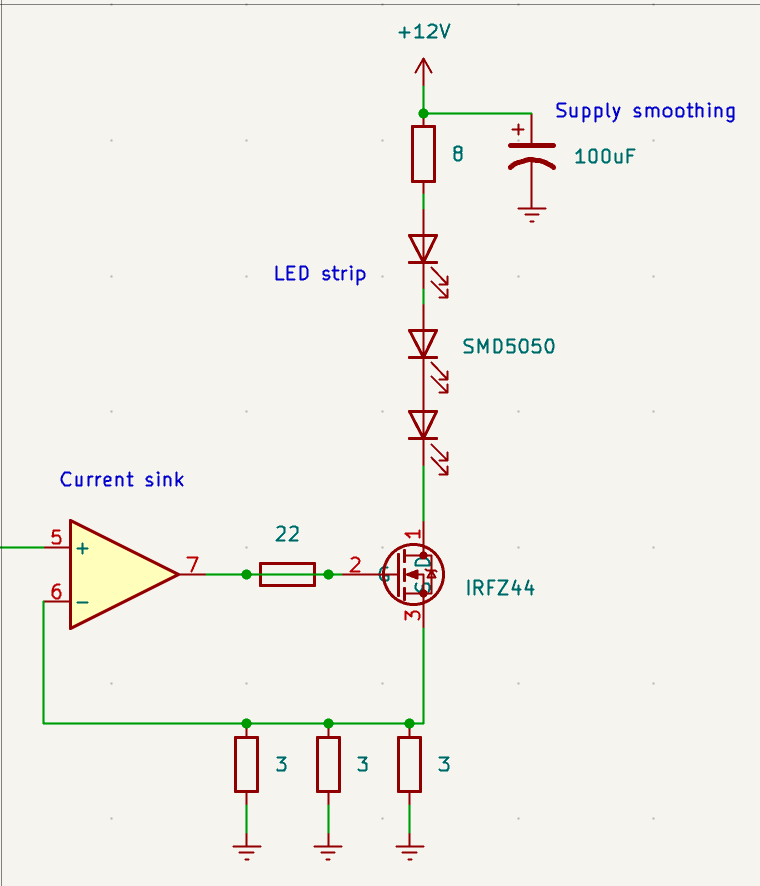
\includegraphics[width=\linewidth]{./figures/LEDsysOut.png}
    \caption{Current sink and LED control stage of the circuit}
    \label{fig:LEDsysOut}
  \end{wrapfigure}

  This means the inverting input is
  \begin{equation*}
    V_{-} = I_{\mathrm{LED}} \cdot R_{S}
  \end{equation*}
  And since the opamp will try to force $V_{-} \approx V_{+} = V_{\mathrm{control}}$:
  \begin{equation*}
    V_{\mathrm{control}} \approx I_{\mathrm{LED}} \cdot R_S \implies I_{\mathrm{LED}} \approx \frac{V_{\mathrm{control}}}{R_S} \approx V_{\mathrm{control}}
  .\end{equation*}
  Hence, the voltage delivered from the low-pass filter will correspond numerically to the amps through the LED strip.

  Here, a smoothing capacitor of \qty{100}{\micro\farad} has been used to smooth the supply to the LED-strip.
  It should also be noted that the \qty{8}{\ohm} resistor drawn on the schematic on \Cref{fig:LEDsysOut} is built into the LED-strip itself.

  The MOSFET functions as a current valve.
  When a larger voltage is supplied to the MOSFET gate from the opamp the MOSFET will allow more current to flow from its source to its drain thereby allowing more current to flow through the LEDs leading to brighter lights. 
  Conversely, if a smaller voltage is supplied to the MOSFET less current will be allowed to run through the LEDs producing dimmer lights. 

  \section{Falstad Simulation}
  Falstad Circuit Simulator has been used extensively during this project to fine-tune the values of different components and verifying ideas for construction.
  The circuit is available on this \href{https://is.gd/hbJ6FC}{Falstad-Link}.
  On \Cref{fig:Falsims}, Falstad simulations for a \qty{200}{\milli\volt} input signal in different scenarios is shown.

  \begin{figure}[ht]
    \centering

    \begin{subfigure}[t]{0.48\linewidth}
      \centering
      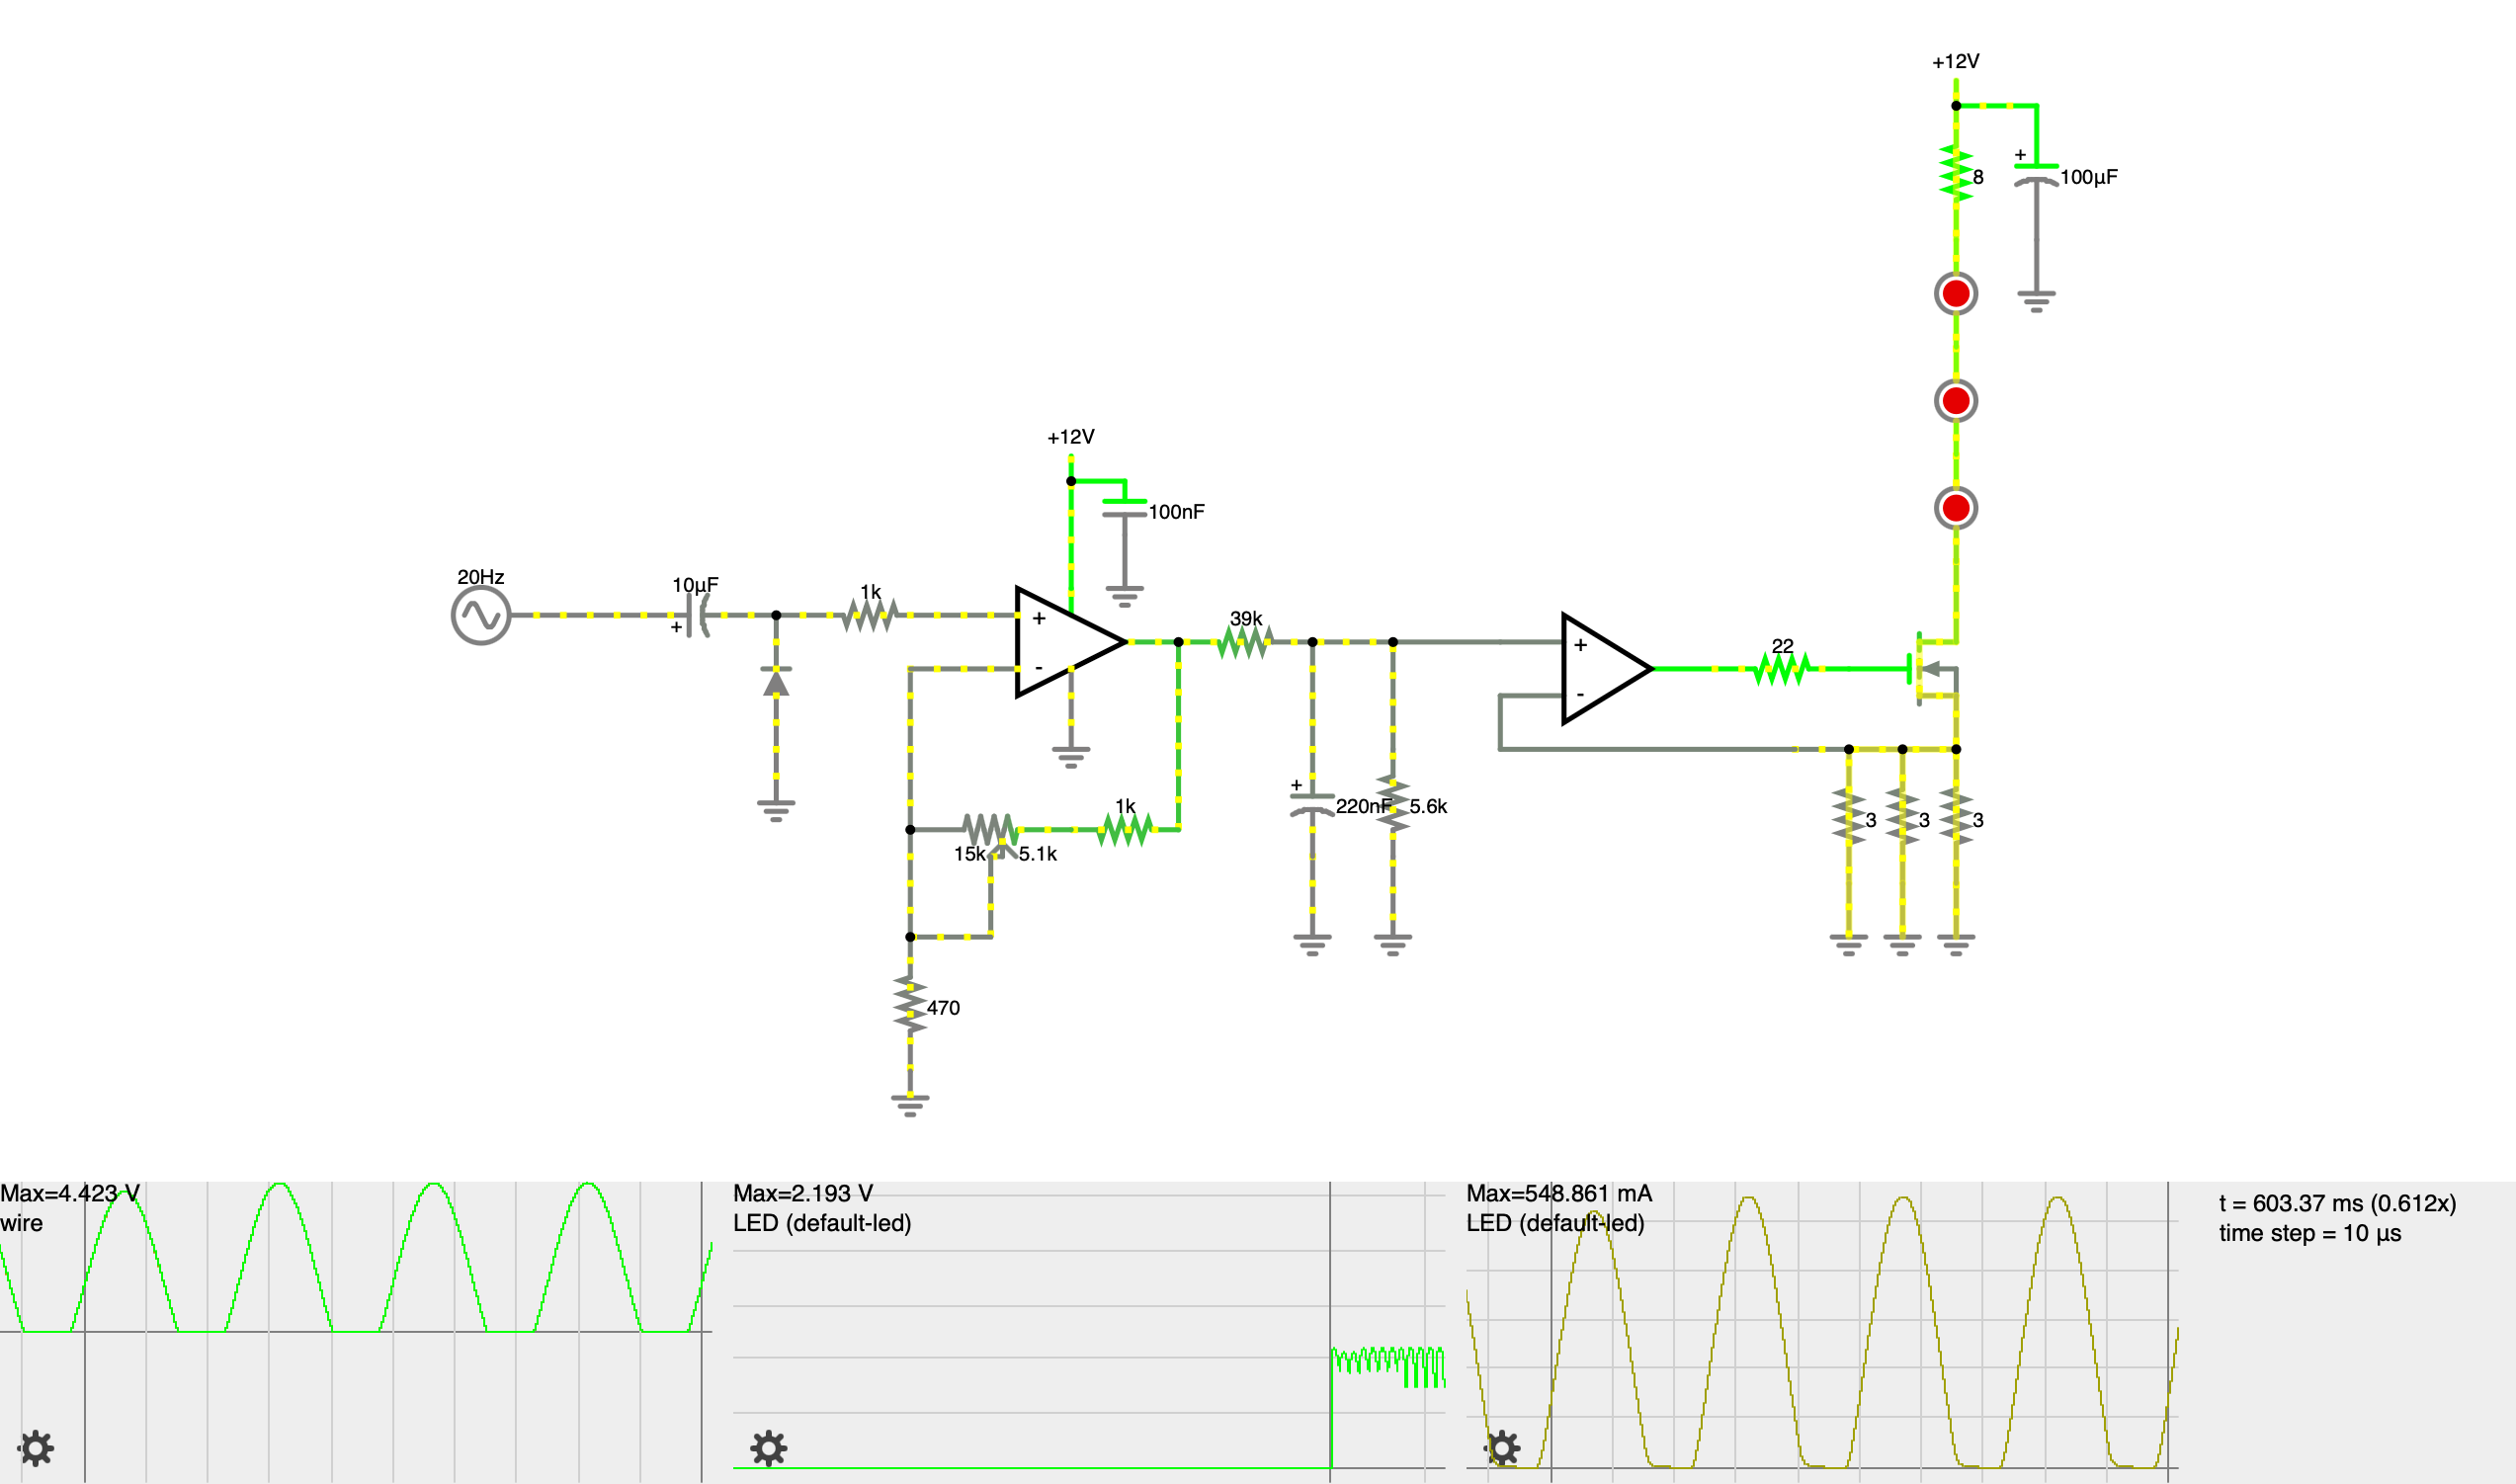
\includegraphics[width=\linewidth]{./figures/20Hz5k.png}
      \caption{\qty{20}{\Hz} signal with pot at \qty{5}{\kilo\ohm}.}
      \label{fig:20Hz5k}
    \end{subfigure}
    \hfill
    \begin{subfigure}[t]{0.48\linewidth}
      \centering
      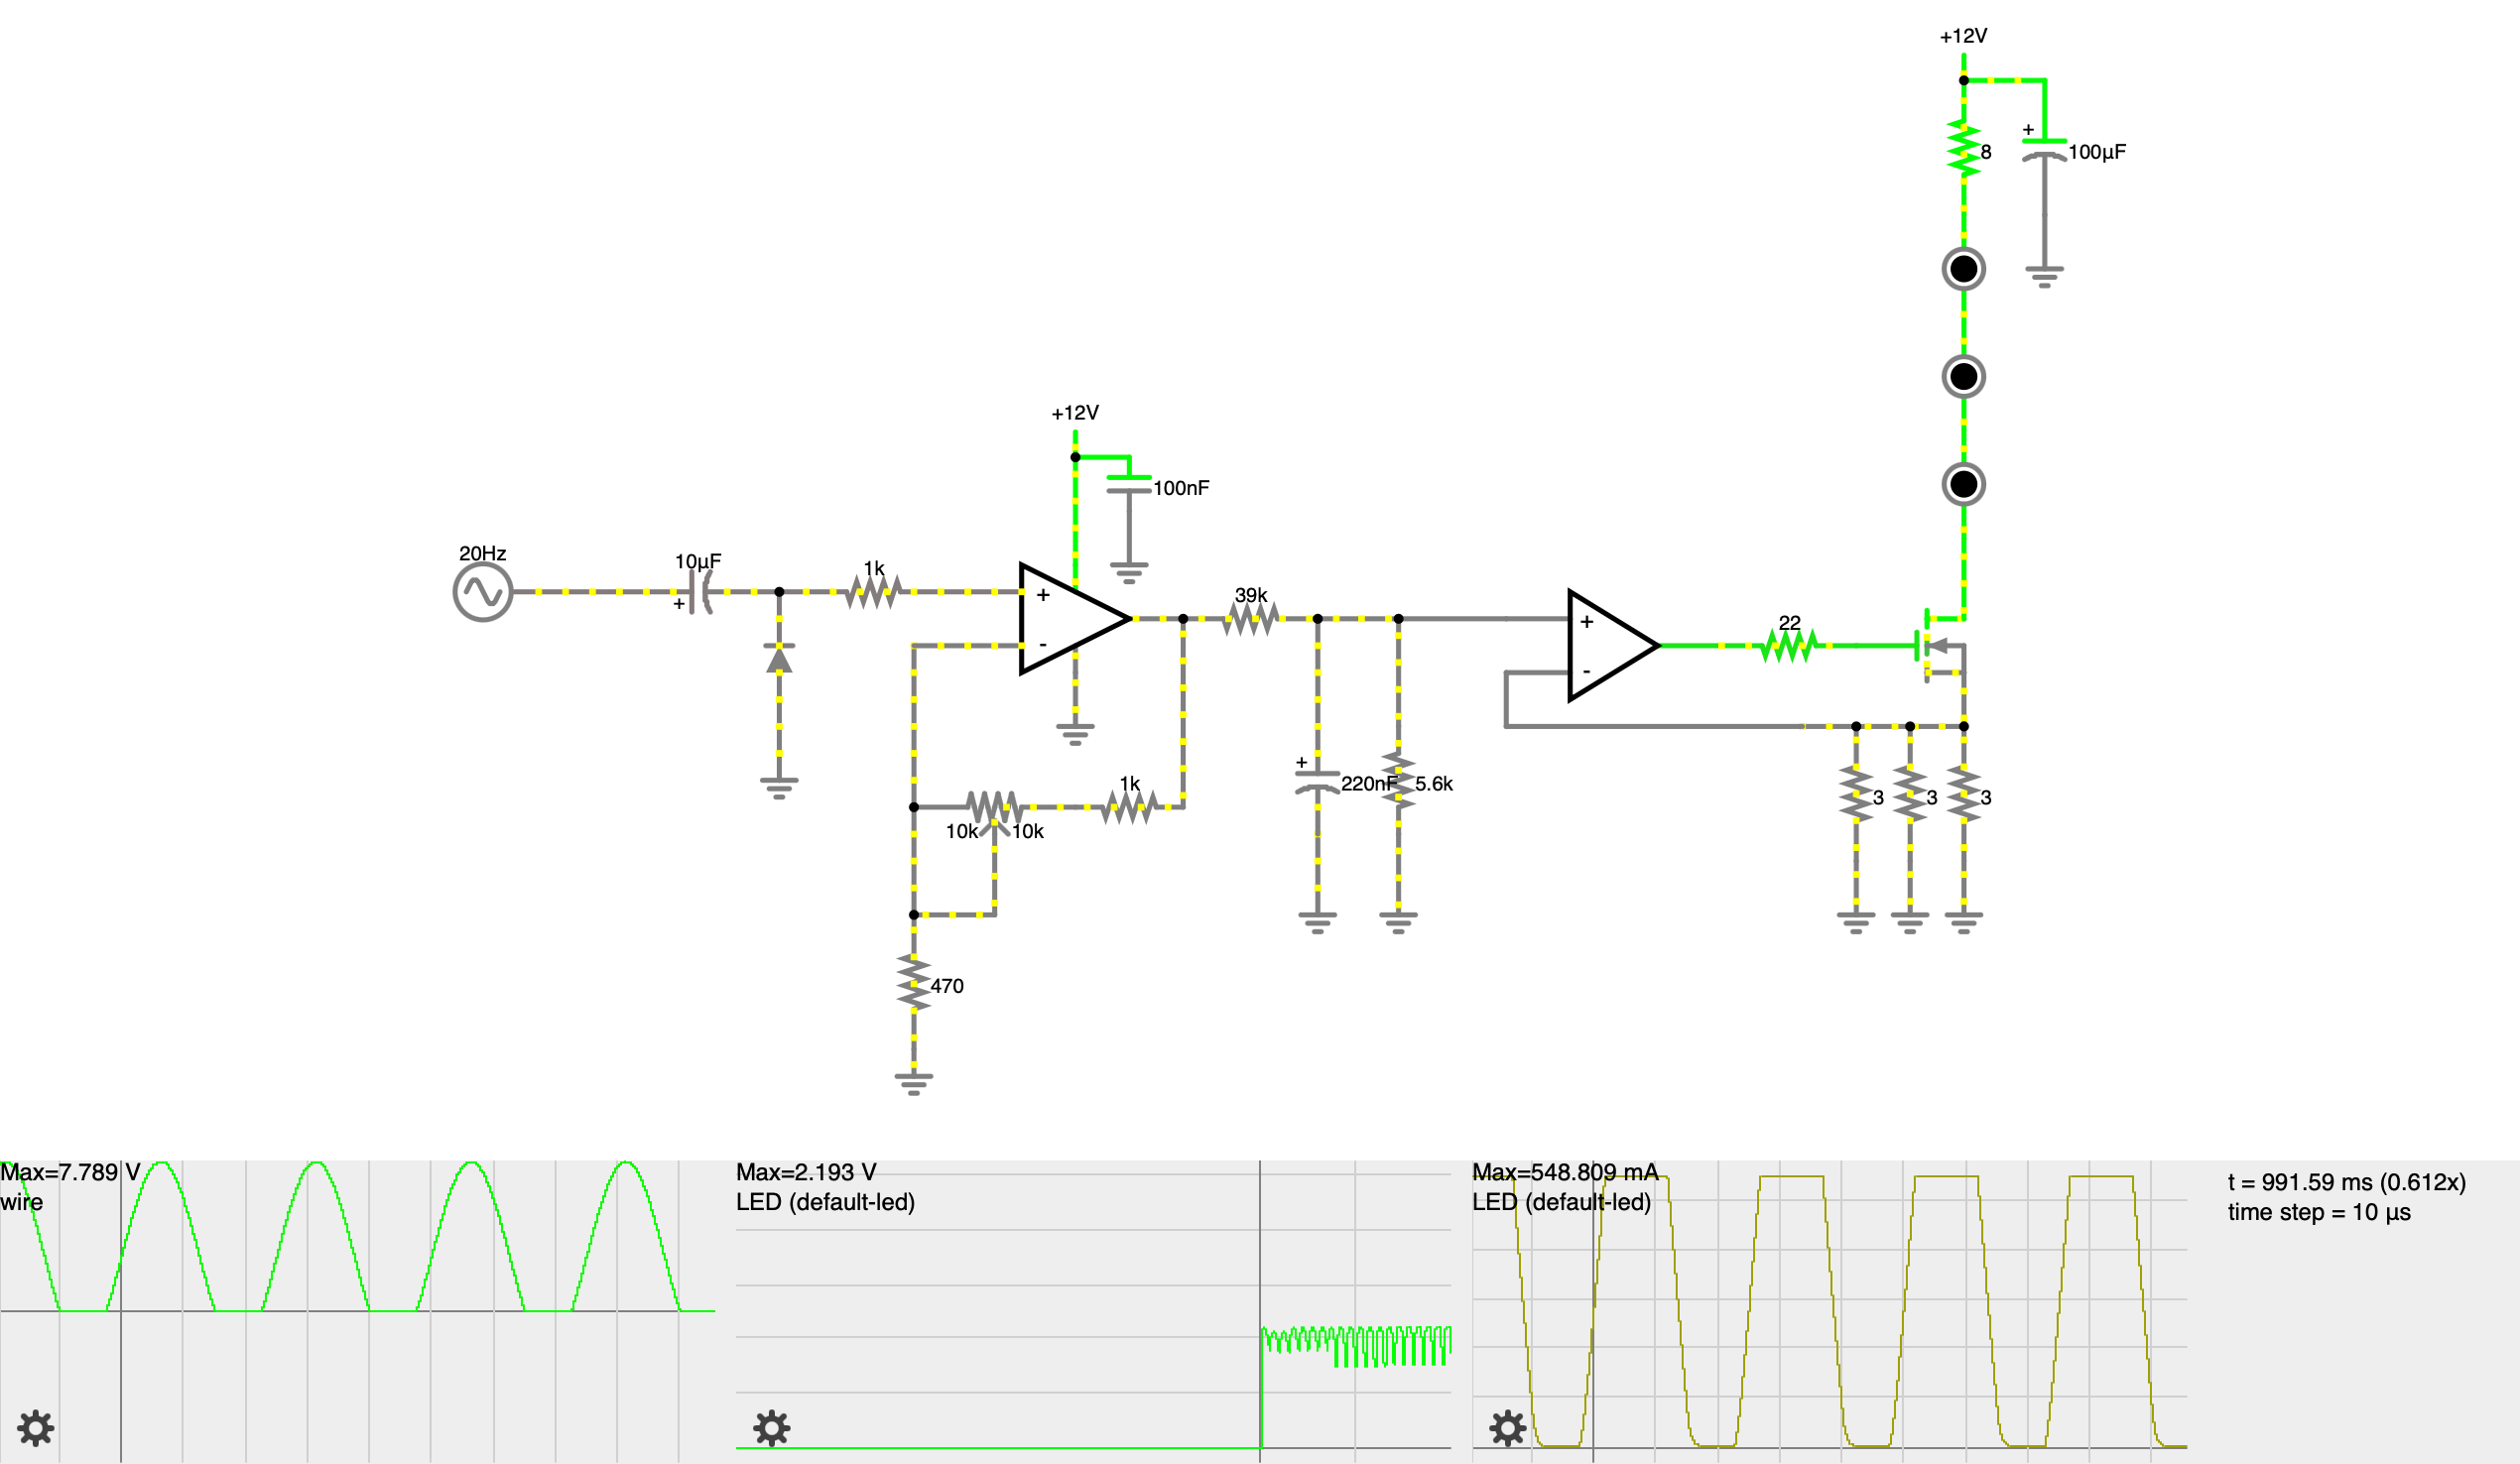
\includegraphics[width=\linewidth]{./figures/20Hz10k.png}
      \caption{\qty{20}{\Hz} signal with pot at \qty{10}{\kilo\ohm}.}
      \label{fig:20Hz10k}
    \end{subfigure}
    \vspace{0.5em}
    \begin{subfigure}[t]{0.48\linewidth}
      \centering
      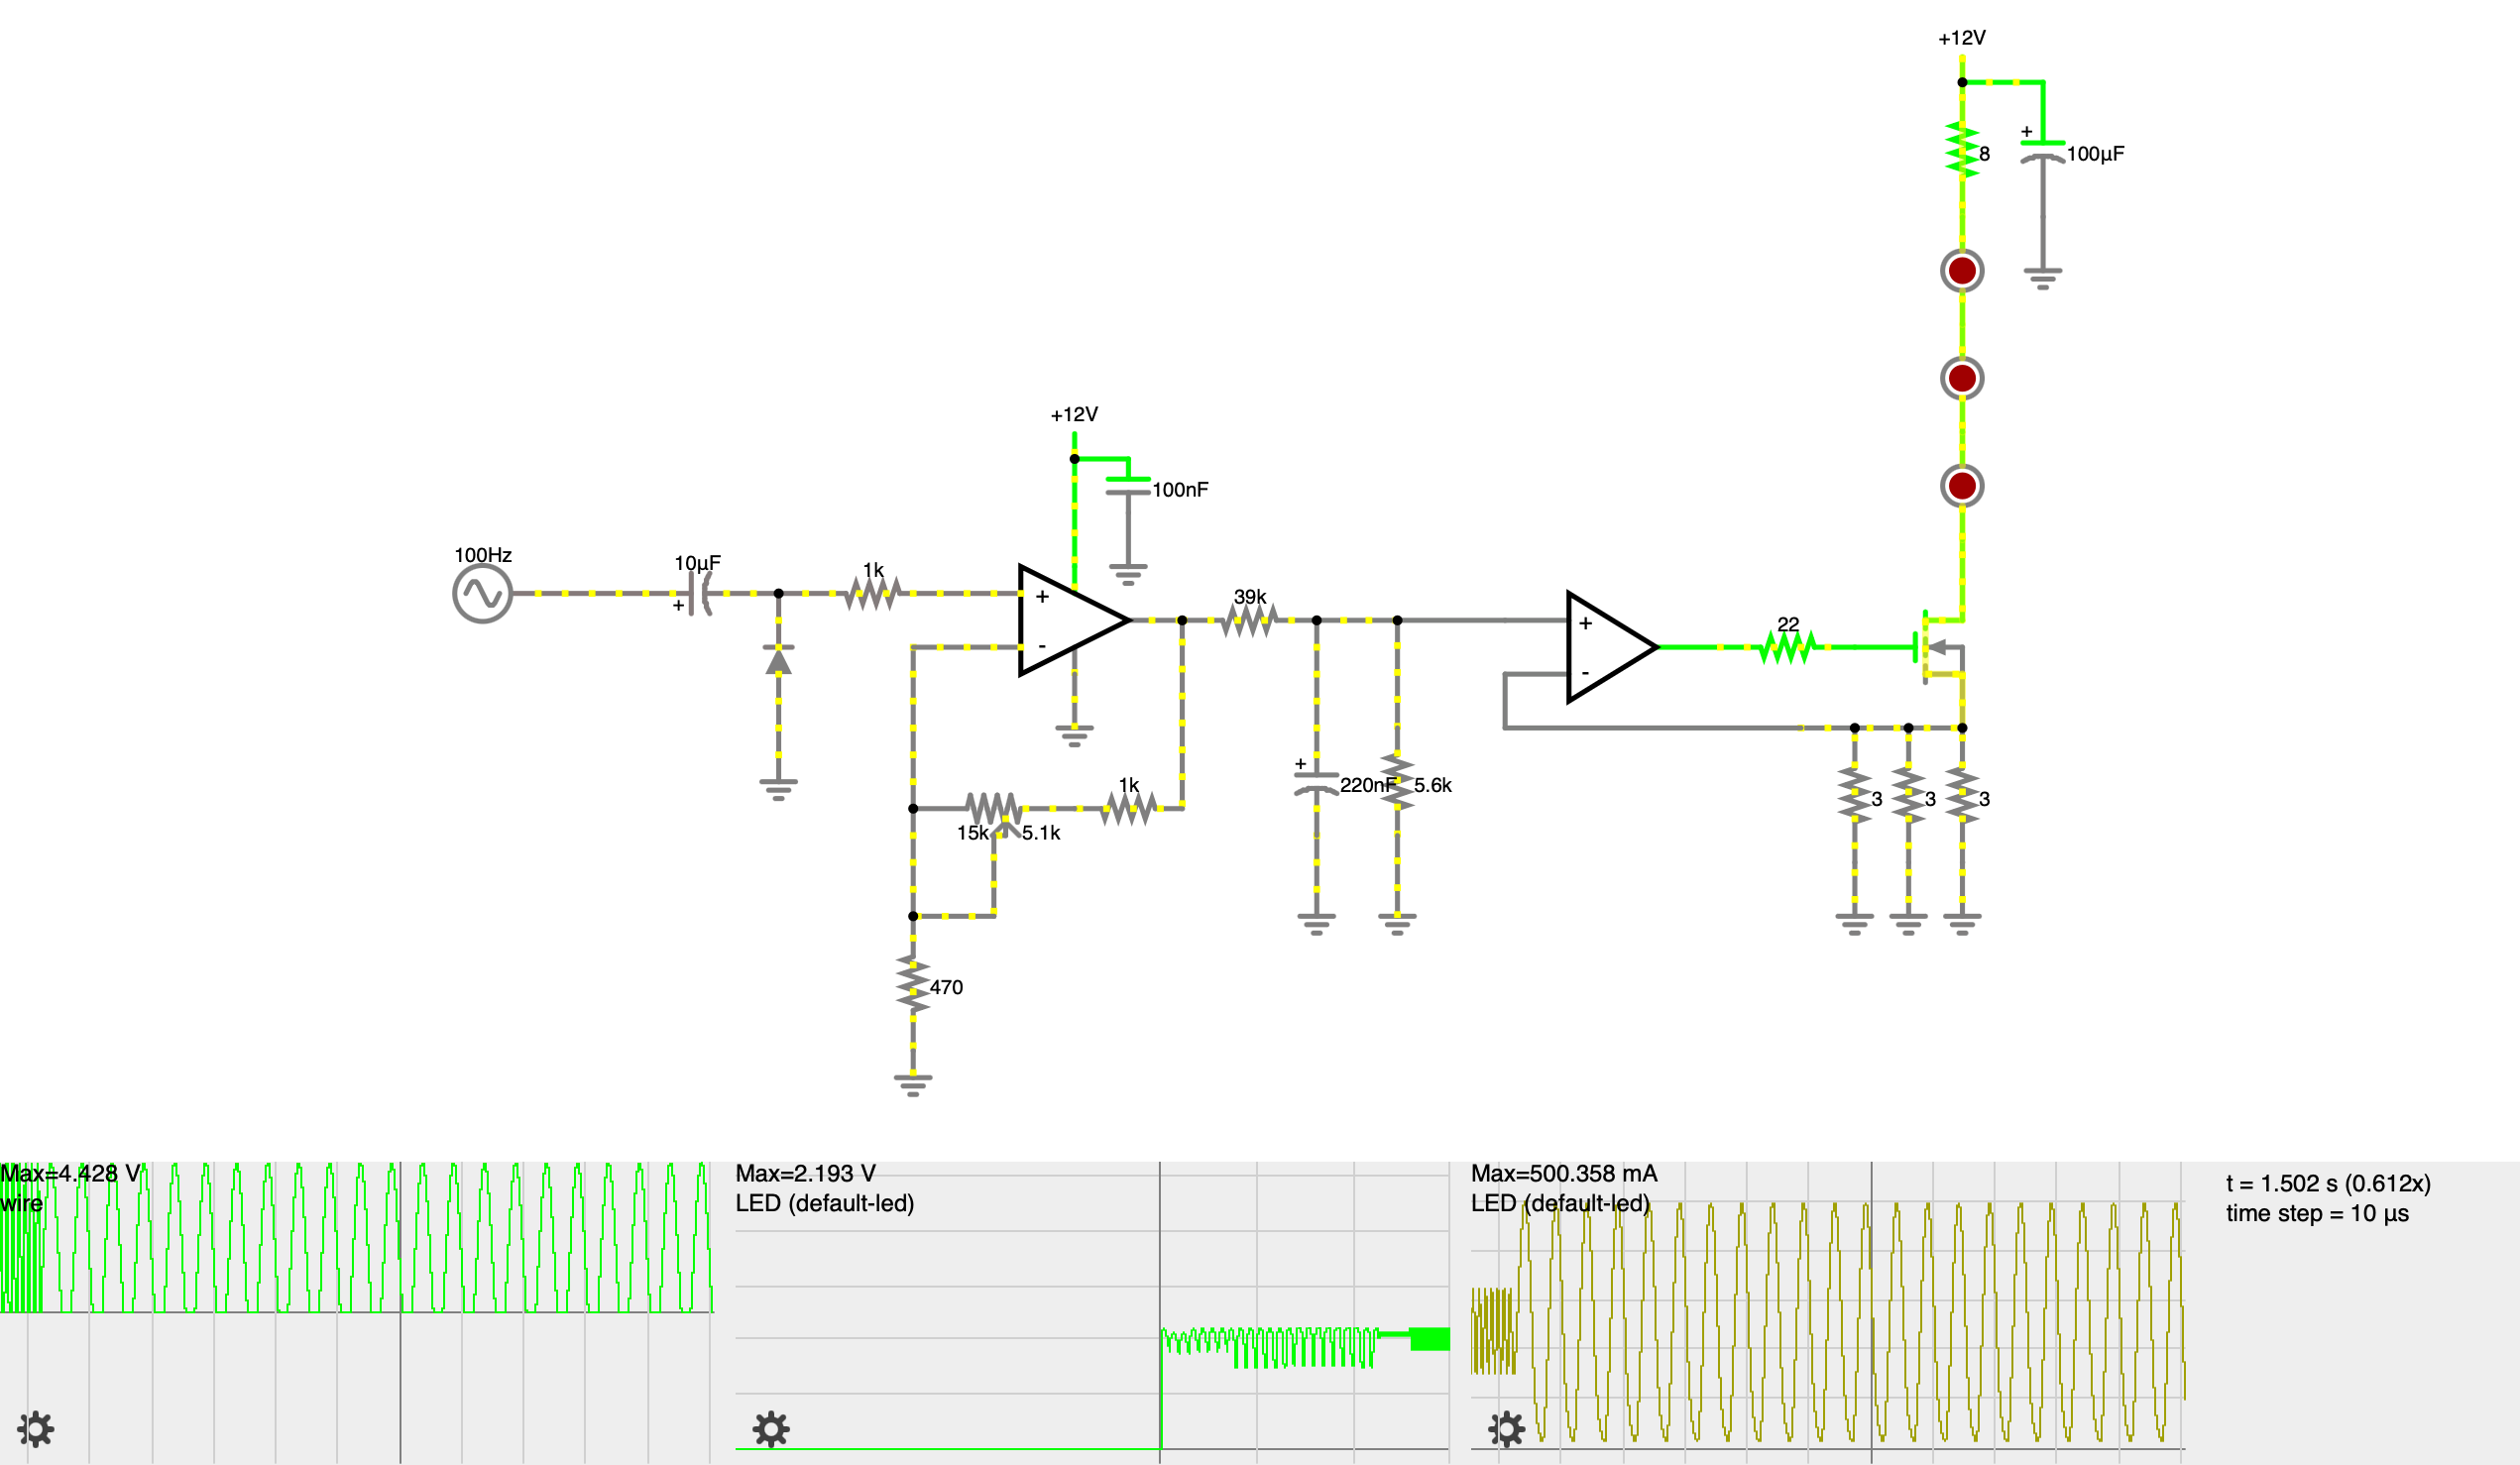
\includegraphics[width=\linewidth]{./figures/100Hz5k.png}
      \caption{\qty{100}{\Hz} signal with pot at \qty{5}{\kilo\ohm}.}
      \label{fig:100Hz5k}
    \end{subfigure}

    \caption{Falstad simulations.}
    \label{fig:Falsims}
  \end{figure}

  On \Cref{fig:20Hz5k,fig:20Hz10k} the input signal is a \qty{20}{\Hz} sine wave.
  These scenarios differ in that the gain potentiometer is at \qty{5}{\kilo\ohm} on \Cref{fig:20Hz5k} and at \qty{10}{\kilo\ohm} on \Cref{fig:20Hz10k}.

  On \Cref{fig:100Hz5k} the input signal is a \qty{100}{\Hz} sine wave.

  \section{Contribution from each member}
  The group work has been split between Benjamin RP, Alfred GA and myself.
  Alfred came up with the idea and in collaboration we made a lot of the initial planning of the circuit and the first considerations about how the circuit should be built.
  After Benjamin also became a part of the group he helped design the KiCad schematics and get the Falstad simulations running.

  I went on vacation in the week before the presentations where most of the circuit was constructed, so Alfred and Benjamin have done the bulk-work of actually producing and testing the physical board in the period where I was only able to communicate with the others through chat-services.

  I joined the group after my vacation again just before we started designing the box for containing the circuit during the presentations.
\end{document}
